\documentclass[journal]{IEEEtran}

% =========================================================================
% PACKAGES
% =========================================================================
\usepackage[utf8]{inputenc}
\usepackage[T1]{fontenc}
\usepackage{amsmath,amssymb,amsfonts}
\usepackage{algorithmic}
\usepackage{graphicx}
\usepackage{textcomp}
\usepackage{xcolor}
\usepackage{booktabs}
\usepackage{cite}
\usepackage{url}
\usepackage{microtype}
\usepackage[hidelinks]{hyperref}
\usepackage{bm}

% Path to graphics
\graphicspath{{figures/}}

% Correct bad hyphenation here
\hyphenation{op-ti-cal net-works semi-conduc-tor phy-sics hy-per-spec-tral emis-si-vi-ty}

\begin{document}

% =========================================================================
% TITLE & AUTHORS
% =========================================================================
\title{Physics-Informed Neural Networks with Sobolev Shape Regularization for Ill-Posed Temperature and Emissivity Separation Across Multispectral and Hyperspectral Thermal Infrared Sensors}

\author{Atilio~Grondona%
\thanks{A. Grondona is with the Department of Remote Sensing and Applied Geosciences. Corresponding author: A. Grondona (e-mail: atilio@example.org).}}

% Header paper mark
\markboth{IEEE Transactions on Geoscience and Remote Sensing,~Vol.~XX, No.~X, Month~2026}%
{Grondona: Physics-Informed Neural Networks with Sobolev Shape Regularization for Thermal Infrared TES}

\maketitle

% =========================================================================
% ABSTRACT & INDEX TERMS
% =========================================================================
\begin{abstract}
The retrieval of land surface temperature (LST) and spectral emissivity (LSE) from thermal infrared (TIR) radiometry constitutes a fundamentally ill-posed inverse problem, governed by an underdetermined system of $N$ radiometric observations and $N+1$ physical unknowns. Operational separation frameworks, such as the standard Temperature and Emissivity Separation (TES) algorithm, rely on empirical power-law relationships between spectral contrast (Min-Max Difference, MMD) and minimum emissivity ($\epsilon_{\min}$). While computationally tractable, these empirical formulations break down over low-contrast targets (e.g., water bodies, dense vegetation, urban asphalt) and introduce systematic errors when applied to complex mineral surfaces with acute reststrahlen absorption doublets. Unconstrained deep neural networks frequently violate thermodynamic boundary conditions or severely oversmooth diagnostic absorption features. In this work, we propose IATIR, a Physics-Informed Neural Network (PINN) framework augmented by discrete 1D Sobolev space ($W^{2,1}$) shape regularization. The architecture employs a shared multi-layer perceptron backbone that branches into decoupled physical heads: a scalar kinetic temperature head constrained by a shifted Softplus activation ($T_s > 200\text{ K}$) and a vector emissivity head bounded by a Sigmoid function ($\bm{\epsilon} \in (0, 1)^N$). To preserve mineral diagnostic morphology, our compound objective function supervises zeroth-order amplitudes via Mean Squared Error (MSE) and Spectral Angle Mapper (SAM), while explicitly penalizing first-order spectral slopes ($\nabla$) and second-order spectral curvatures ($\nabla^2$) under an $L_1$ Total Variation prior. Validated against completely held-out pristine ``Golden Target'' mineral endmembers across both the 256-channel Hyperspectral Thermal Emission Spectrometer (HyTES) and the 5-band Advanced Spaceborne Thermal Emission and Reflection Radiometer (ASTER), our framework reduces second-order spectral curvature error by 79.7\% ($0.03849 \rightarrow 0.00782$), decreases spectral angle mapper (SAM) deviation by 49.3\% ($6.640^\circ \rightarrow 3.366^\circ$), and cuts kinetic surface temperature error by 42.4\% ($2.500\text{ K} \rightarrow 1.441\text{ K}$), reaching sub-Kelvin precision on key silicates ($\Delta T = 0.388\text{ K}$ for kaolinite and $0.902\text{ K}$ for feldspar). The approach establishes a scalable, physically consistent inversion paradigm directly applicable to next-generation spaceborne TIR missions, including NASA SBG and Copernicus LSTM.
\end{abstract}

\begin{IEEEkeywords}
Thermal infrared (TIR), temperature and emissivity separation (TES), physics-informed neural networks (PINNs), Sobolev training, shape regularization, HyTES, ASTER, radiative transfer equation (RTE), remote sensing.
\end{IEEEkeywords}

\IEEEpeerreviewmaketitle

% =========================================================================
% SECTION I: INTRODUCTION
% =========================================================================
\section{Introduction}
\IEEEPARstart{L}{and} Surface Temperature (LST) and Land Surface Emissivity (LSE) are fundamental Essential Climate Variables (ECVs) governing surface-atmosphere energy exchanges, evapotranspiration rates, geothermal monitoring, urban heat island dynamics, and lithological mapping \cite{salisbury1992emissivity, hecker2011thermal, cawsenicholson2021nasa}. Recovering surface kinetic temperature $T_s$ and spectral emissivity $\bm{\epsilon} = [\epsilon_1, \dots, \epsilon_N]^T$ from spaceborne or airborne thermal infrared (TIR, 8--14~$\mu\text{m}$) radiometry is historically hampered by an intractable algebraic limitation: a radiometer equipped with $N$ spectral channels records $N$ top-of-atmosphere (TOA) radiance values, yet the inversion system must simultaneously resolve $N+1$ independent physical parameters ($N$ channel emissivities plus $T_s$).

To circumvent this underdetermined condition, classical operational algorithms enforce empirical approximations. The seminal Temperature and Emissivity Separation (TES) algorithm developed for ASTER \cite{gillespie1998temperature}, and subsequently adapted for the MODIS MOD21 product \cite{hulley2015mod21}, ECOSTRESS on the International Space Station \cite{hulley2018ecostress}, and the airborne Hyperspectral Thermal Emission Spectrometer (HyTES) \cite{hulley2012hytes, hook2013hyperspectral}, relies on the empirical Maximum-Minimum Difference (MMD) relationship:
\begin{equation}
\epsilon_{\min} = a - b \cdot (\text{MMD})^c
\label{eq:mmd_empirical}
\end{equation}
where $\text{MMD} = \max(\beta_i) - \min(\beta_i)$ is computed from relative emissivity ratios $\beta_i$. Although robust over typical terrestrial soils, empirical MMD formulations exhibit acute physical vulnerabilities: they fail catastrophically over low-contrast graybodies ($\text{MMD} \to 0$) where empirical power-law slopes diverge, and introduce substantial uncertainty when unmodeled mineral mixtures or variable atmospheric attenuation violate laboratory calibration baselines \cite{perezplanells2017retrieval}.

With the recent paradigm shift toward Physics-Informed Machine Learning (PIML) \cite{raissi2019physics, kashinath2021physics}, deep learning architectures have demonstrated remarkable capability in solving non-linear inverse problems in radiative transfer \cite{mishra2021physics} and optical metamaterials \cite{chen2020physics}. However, deploying standard unconstrained deep neural networks to TIR temperature-emissivity retrieval exposes three critical failure modes:
\begin{enumerate}
    \item \textbf{Thermodynamic Inversion Anomalies:} Standard unconstrained linear or polynomial output layers frequently predict negative kinetic temperatures ($T_s < 0\text{ K}$) or emissivities outside the physically permissible interval $[0, 1]$, violating Kirchhoff's radiation law.
    \item \textbf{Spectral Oversmoothing ($L_2$ Loss Artifact):} Classical Mean Squared Error (MSE) objective functions penalize deviations quadratically across the batch, driving the model toward the conditional expectation $\mathbb{E}[\bm{\epsilon}|\bm{L}_{\text{obs}}]$. This acts as a severe low-pass filter over the spectral domain, flattening acute mineral diagnostic absorption features (such as the quartz reststrahlen band at $8.2\text{--}8.6\ \mu\text{m}$ and the kaolinite Al-OH doublet at $9.6\text{--}10.1\ \mu\text{m}$).
    \item \textbf{Cross-Sensor Discontinuity:} Existing inversion schemes are rigidly engineered either for multispectral instruments (e.g., ASTER, 5 bands) or hyperspectral spectrometers (e.g., HyTES, 256 bands), lacking architectural scalability across varying spectral resolutions.
\end{enumerate}

To overcome these structural limitations, this study presents \textbf{IATIR}, a multi-head Physics-Informed Neural Network integrated with discrete 1D Sobolev ($W^{2,1}$) regularization \cite{czarnecki2017sobolev, son2021sobolev}. The primary contributions and novelties of this paper are summarized as follows:
\begin{itemize}
    \item \textbf{Thermodynamically Guaranteed Architecture:} We introduce parameter-free, strictly bounded activation functions ($T_s > 200\text{ K}$ via a shifted Softplus layer and $\epsilon_i \in (0, 1)$ via Sigmoid) that guarantee thermodynamic compliance across all gradient updates without unphysical clipping.
    \item \textbf{Discrete 1D Sobolev ($W^{2,1}$) Shape Regularization:} We establish a functional analysis framework supervising first-order spectral slopes ($\nabla \bm{\epsilon}$) and second-order spectral curvatures ($\nabla^2 \bm{\epsilon}$) under an $L_1$ norm. This acts as a Total Variation regularizer, preserving sharp reststrahlen inflection walls while eliminating spurious noise oscillations.
    \item \textbf{Curriculum Refinement \& Clean-Room Validation:} We implement a two-stage curriculum training protocol (generalist noisy base model followed by low-learning-rate high-fidelity fine-tuning) rigorously evaluated against pristine, quarantined ``Golden Target'' mineral endmembers to prevent spatial and spectral data leakage.
    \item \textbf{Cross-Resolution Sensor Scalability:} We demonstrate seamless operational generalization across both 256-band HyTES and 5-band ASTER architectures, providing sub-Kelvin thermal accuracy and sub-millisecond inference speeds directly relevant to upcoming Earth Observation missions including NASA SBG \cite{cawsenicholson2021nasa} and ESA Copernicus LSTM \cite{koetz2018high}.
\end{itemize}

% =========================================================================
% SECTION II: THEORETICAL BASELINE & RADIATIVE TRANSFER
% =========================================================================
\section{Physical Principles and Radiative Transfer Baseline}

\subsection{Thermal Infrared Radiative Transfer Formulation}
The spectral radiance observed at the top of the atmosphere (TOA) by a downward-looking remote sensor viewing an opaque, Lambertian terrestrial surface under clear-sky conditions at wavelength $\lambda$ is governed by the thermal radiative transfer equation (RTE) \cite{salisbury1992emissivity, perezplanells2017retrieval}:
\begin{equation}
L_{\text{obs}}(\lambda) = \tau(\lambda)\epsilon(\lambda)B(\lambda, T_s) + L_{\text{up}}(\lambda) + \tau(\lambda)[1 - \epsilon(\lambda)]L_{\text{down}}(\lambda)
\label{eq:rte}
\end{equation}
where:
\begin{itemize}
    \item $L_{\text{obs}}(\lambda)$ is the TOA spectral radiance $[\text{W}\cdot\text{m}^{-2}\cdot\text{sr}^{-1}\cdot\mu\text{m}^{-1}]$,
    \item $\tau(\lambda)$ denotes the total spectral atmospheric transmittance along the surface-to-sensor optical path,
    \item $\epsilon(\lambda)$ represents the directional surface spectral emissivity,
    \item $T_s$ is the true surface kinetic temperature $[\text{K}]$,
    \item $B(\lambda, T_s)$ is Planck's blackbody radiation function at temperature $T_s$,
    \item $L_{\text{up}}(\lambda)$ is the upward atmospheric path radiance emitted directly toward the sensor,
    \item $L_{\text{down}}(\lambda) = F_{\text{down}}(\lambda)/\pi$ is the effective hemispherical downwelling atmospheric sky radiance reflected by the surface.
\end{itemize}

Planck's blackbody spectral distribution function is analytically expressed as:
\begin{equation}
B(\lambda, T_s) = \frac{c_1}{\lambda^5 \left[\exp\left(\frac{c_2}{\lambda T_s}\right) - 1\right]}
\label{eq:planck}
\end{equation}
where $c_1 = 2hc^2 = 1.19104 \times 10^8\ \text{W}\cdot\mu\text{m}^4\cdot\text{m}^{-2}\cdot\text{sr}^{-1}$ denotes the first radiation constant, and $c_2 = hc/k = 1.43877 \times 10^4\ \mu\text{m}\cdot\text{K}$ represents the second radiation constant ($h$, $c$, and $k$ being Planck's constant, the speed of light in vacuum, and Boltzmann's constant, respectively).

\subsection{Channel Integration and Spectral Response Functions}
Real-world optical sensors acquire radiance through finite spectral bandpasses characterized by normalized Spectral Response Functions (SRFs). For an instrument channel $j \in \{1, \dots, N\}$ with normalized filter response $S_j(\lambda)$ bounded over wavelength interval $[\lambda_{j,\min}, \lambda_{j,\max}]$, the effective bandpass-averaged radiance $L_j$ and surface emissivity $\epsilon_j$ are defined by the Fredholm integral of the first kind:
\begin{equation}
L_j = \frac{\int_{\lambda_{j,\min}}^{\lambda_{j,\max}} L_{\text{obs}}(\lambda) S_j(\lambda) \, d\lambda}{\int_{\lambda_{j,\min}}^{\lambda_{j,\max}} S_j(\lambda) \, d\lambda}
\label{eq:channel_rad}
\end{equation}
\begin{equation}
\epsilon_j = \frac{\int_{\lambda_{j,\min}}^{\lambda_{j,\max}} \epsilon(\lambda) S_j(\lambda) \, d\lambda}{\int_{\lambda_{j,\min}}^{\lambda_{j,\max}} S_j(\lambda) \, d\lambda}
\label{eq:channel_eps}
\end{equation}
Consequently, given $N$ discrete radiometric measurements $\bm{L}_{\text{obs}} = [L_1, \dots, L_N]^T \in \mathbb{R}^N$, the inversion system must simultaneously retrieve the vector of channel emissivities $\bm{\epsilon} = [\epsilon_1, \dots, \epsilon_N]^T \in [0, 1]^N$ and the scalar surface kinetic temperature $T_s \in \mathbb{R}^+$. Because there are $N$ equations and $N+1$ unknowns, the system possesses an infinite number of exact mathematical solutions in the absence of additional physical constraints.

\subsection{The Empirical MMD Bottleneck in Classical TES}
To resolve this underdetermined algebraic defect, operational algorithms such as the ASTER/MODIS Temperature and Emissivity Separation (TES) algorithm \cite{gillespie1998temperature, hulley2015mod21, hulley2018ecostress} execute a three-step heuristic:
\begin{enumerate}
    \item \textbf{NEM Module:} Initial estimates of surface temperature and relative emissivities are computed by assuming an initial maximum emissivity $\epsilon_{\max} \approx 0.96$--$0.99$.
    \item \textbf{Ratio Module:} Normalizing channel emissivities by their spectral mean yields relative emissivity ratios $\beta_j$:
    \begin{equation}
    \beta_j = \frac{\epsilon_j}{\frac{1}{N}\sum_{k=1}^N \epsilon_k} \approx \frac{L_j - L_{\text{up},j}}{\frac{1}{N}\sum_{k=1}^N (L_k - L_{\text{up},k})}
    \end{equation}
    \item \textbf{MMD Module:} The spectral contrast (Min-Max Difference, MMD) is extracted as $\text{MMD} = \max(\beta_j) - \min(\beta_j)$. The minimum absolute emissivity $\epsilon_{\min}$ is then predicted via an empirical power-law regression calibrated on laboratory spectral libraries:
    \begin{equation}
    \epsilon_{\min} = a - b \cdot (\text{MMD})^c
    \label{eq:mmd_regression}
    \end{equation}
\end{enumerate}
Despite its widespread operational deployment in the MOD21 and ECOSTRESS products, the empirical MMD formulation introduces critical physical vulnerabilities:
\begin{itemize}
    \item \textbf{Graybody Singularity:} Over surfaces with low spectral contrast (e.g., open water, snow, dense vegetation, wet soils), $\text{MMD} \to 0$. Under small radiometric calibration noise or atmospheric correction residuals, $\text{MMD}$ fluctuates erratically, causing the power law in (\ref{eq:mmd_regression}) to output unphysical emissivities exceeding unity or severely overestimating $T_s$.
    \item \textbf{Mineral Outliers:} For mineral surfaces exhibiting complex multi-band reststrahlen features (such as carbonates and altered phyllosilicates \cite{hecker2011thermal}), the true relationship between $\text{MMD}$ and $\epsilon_{\min}$ deviates substantially from the global regression curve, yielding systematic residual errors of $1.0\text{ to }2.0\text{ K}$ \cite{perezplanells2017retrieval}.
\end{itemize}

\subsection{Spectral Library Grounding and Kirchhoff's Law}
To ground the learning procedure on pristine physical reality, all baseline spectral emissivities are derived from high-precision laboratory directional hemispherical reflectance (DHR) measurements compiled in the ECOSTRESS and ASTER Spectral Libraries \cite{baldridge2009aster, salisbury1992emissivity}. Under Kirchhoff's law of thermal radiation for an opaque, optically thick medium in thermodynamic equilibrium, directional spectral emissivity is strictly related to spectral reflectance $R(\lambda)$ by:
\begin{equation}
\epsilon(\lambda) = 1.0 - R(\lambda)
\label{eq:kirchhoff}
\end{equation}
All laboratory spectra were processed across the thermal infrared atmospheric window ($8.0\text{ to }12.0\ \mu\text{m}$) and resampled to the sensor SRFs via (\ref{eq:channel_eps}).

\subsection{Atmospheric Transfer Database Generation}
Atmospheric parameter triples $\{\tau(\lambda), L_{\text{up}}(\lambda), L_{\text{down}}(\lambda)\}$ were generated using automated MODTRAN~6 radiative transfer simulations \cite{berk2014modtran6}. The simulation grid systematically perturbed:
\begin{itemize}
    \item Column Water Vapor (CWV) from $0.5\text{ to }4.5\ \text{g}\cdot\text{cm}^{-2}$ in increments of $0.5\ \text{g}\cdot\text{cm}^{-2}$,
    \item Surface kinetic temperatures $T_s$ from $280\text{ to }330\text{ K}$ in increments of $5\text{ K}$,
    \item Standard atmospheric profiles (Mid-Latitude Summer, US Standard 1976) with rural aerosol extinction ($23\text{ km}$ visibility).
\end{itemize}

% =========================================================================
% SECTION III: METHODOLOGY & SOBOLEV PINN ARCHITECTURE
% =========================================================================
\section{Physics-Informed Architecture with Sobolev Shape Regularization}

\subsection{Multi-Head PINN Topology and Thermodynamic Enforcements}
The IATIR neural architecture is engineered as a bifurcated multi-head network. Rather than treating $T_s$ and $\bm{\epsilon}$ as mutually independent unconstrained outputs, the network extracts shared latent representations from the input radiance vector and processes them through specialized, physically constrained output heads.

\subsubsection{Shared Latent Backbone}
The input feature vector consists of the observed radiance $\bm{L}_{\text{obs}} \in \mathbb{R}^N$. The feature extractor comprises a multi-layer perceptron (MLP) with 4 fully connected dense layers, each containing 512 hidden units:
\begin{align}
\bm{h}_0 &= \bm{L}_{\text{obs}} \in \mathbb{R}^N \\
\bm{h}_l &= \text{GELU}(\bm{W}_l \bm{h}_{l-1} + \bm{b}_l), \quad l \in \{1, 2, 3, 4\}
\end{align}
where $\bm{W}_l \in \mathbb{R}^{512 \times 512}$ and $\bm{b}_l \in \mathbb{R}^{512}$ (with $\bm{W}_1 \in \mathbb{R}^{512 \times N}$).

We specifically deploy the Gaussian Error Linear Unit (GELU) \cite{raissi2019physics}:
\begin{equation}
\text{GELU}(x) = x \cdot \Phi(x) = x \cdot P(X \le x), \quad X \sim \mathcal{N}(0, 1)
\end{equation}
Unlike standard piecewise-linear Rectified Linear Units (ReLU), which exhibit discontinuous first derivatives ($\nabla \text{ReLU}(0)$ undefined) and zero second derivatives ($\nabla^2 \text{ReLU} \equiv 0$), GELU is a smooth, continuously differentiable ($C^\infty$) activation function. This mathematical property is mandatory for Sobolev regularized backpropagation, as gradient flows through $\nabla$ and $\nabla^2$ operator graphs require non-zero, stable second-order derivative gradients during optimization.

\subsubsection{Decoupled Physical Output Heads}
From the final latent state $\bm{h}_4 \in \mathbb{R}^{512}$, two decoupled prediction heads enforce strict thermodynamic boundary conditions:
\begin{enumerate}
    \item \textbf{Kinetic Surface Temperature Head ($T_s$):} Standard terrestrial surface temperatures rarely drop below $200\text{ K}$. To eliminate unphysical negative temperatures or hyper-cold convergence traps, we formulate an analytical Softplus layer with an explicit physical pedestal:
    \begin{equation}
    \hat{T}_s = \text{Softplus}(\bm{w}_T^T \bm{h}_4 + b_T) + 200.0 = \ln\left(1 + \exp(\bm{w}_T^T \bm{h}_4 + b_T)\right) + 200.0
    \label{eq:temp_head}
    \end{equation}
    where $\bm{w}_T \in \mathbb{R}^{512}$ and $b_T \in \mathbb{R}$. Equation~(\ref{eq:temp_head}) guarantees $\hat{T}_s > 200.0\text{ K}$ everywhere while remaining strictly convex and smooth.
    
    \item \textbf{Spectral Emissivity Head ($\bm{\epsilon}$):} Under Kirchhoff's radiation law and conservation of energy, the emissivity of an opaque non-scattering medium is strictly bounded between zero and unity. We map the spectral output through an element-wise Sigmoid function:
    \begin{equation}
    \hat{\bm{\epsilon}} = \sigma(\bm{W}_\epsilon \bm{h}_4 + \bm{b}_\epsilon) = \frac{1}{1 + \exp(-(\bm{W}_\epsilon \bm{h}_4 + \bm{b}_\epsilon))} \in (0, 1)^N
    \label{eq:eps_head}
    \end{equation}
    where $\bm{W}_\epsilon \in \mathbb{R}^{N \times 512}$ and $\bm{b}_\epsilon \in \mathbb{R}^N$.
\end{enumerate}

\subsection{Discrete 1D Sobolev Space Formulation ($W^{2,1}$)}
The fundamental limitation of standard deep learning regression models in mineral spectroscopy is their reliance on zeroth-order $L_2$ loss metrics:
\begin{equation}
\mathcal{L}_{\text{MSE}}(\bm{\epsilon}, \hat{\bm{\epsilon}}) = \frac{1}{N}\sum_{i=1}^N (\epsilon_i - \hat{\epsilon}_i)^2
\label{eq:mse_def}
\end{equation}
Because the $L_2$ norm minimizes the expected variance across training batches, it acts as a low-pass filter over the spectral domain. When tasked with inverting noisy radiances, unregularized networks converge to the conditional mean of the emissivity manifold, severely flattening the narrow, high-frequency absorption doublets characteristic of silicates and clays.

To penalize spectral flattening, we formulate the loss function over the discrete Sobolev space $W^{2,1}(\Omega)$. In functional analysis, the classical Sobolev norm of order $k$ in $L^p$ space is defined by \cite{czarnecki2017sobolev, son2021sobolev}:
\begin{equation}
\|u\|_{W^{k,p}(\Omega)} = \left( \sum_{|\alpha| \le k} \|D^\alpha u\|_{L^p(\Omega)}^p \right)^{1/p}
\end{equation}
Setting $k=2$ and $p=1$ establishes the continuous Sobolev space $W^{2,1}(\Omega)$, whose norm combines function values, first derivatives (slopes), and second derivatives (curvatures):
\begin{equation}
\|f\|_{W^{2,1}} = \int_\Omega |f(\lambda)| \, d\lambda + \int_\Omega \left|\frac{df}{d\lambda}\right| \, d\lambda + \int_\Omega \left|\frac{d^2f}{d\lambda^2}\right| \, d\lambda
\label{eq:continuous_sobolev}
\end{equation}

For a discrete sensor bandpass vector with channel centers $\lambda_1 < \lambda_2 < \dots < \lambda_N$, we construct the discrete 1D finite-difference Sobolev operators:
\begin{align}
\nabla \epsilon_i &= \epsilon_{i+1} - \epsilon_i, \quad i \in \{1, \dots, N-1\} \label{eq:grad_def} \\
\nabla^2 \epsilon_i &= \nabla \epsilon_{i+1} - \nabla \epsilon_i = \epsilon_{i+2} - 2\epsilon_{i+1} + \epsilon_i, \quad i \in \{1, \dots, N-2\} \label{eq:curv_def}
\end{align}

We specifically select the $L_1$ norm (rather than $L_2$) for the differential operators $\nabla$ and $\nabla^2$. In mathematical optimization, the $L_1$ norm promotes sparsity in the residual gradient domain, analogous to Total Variation (TV) regularization. This allows the network to maintain steep, localized mineral absorption walls (e.g., the quartz reststrahlen inflection at $8.2\ \mu\text{m}$) without penalizing true physical discontinuity.

Furthermore, to guarantee directional alignment of the spectral vectors independent of absolute scaling, we incorporate the Spectral Angle Mapper (SAM) loss:
\begin{equation}
\mathcal{L}_{\text{SAM}}(\bm{\epsilon}, \hat{\bm{\epsilon}}) = 1 - \frac{\sum_{i=1}^N \epsilon_i \hat{\epsilon}_i}{\sqrt{\sum_{i=1}^N \epsilon_i^2} \sqrt{\sum_{i=1}^N \hat{\epsilon}_i^2} + \delta}
\label{eq:sam_def}
\end{equation}
where $\delta = 10^{-8}$ prevents division by zero.

The complete composite objective function optimized during training is formulated as:
\begin{align}
\mathcal{L}_{\text{Total}} = &\; w_e \mathcal{L}_{\text{MSE}}(\bm{\epsilon}, \hat{\bm{\epsilon}}) + w_t \mathcal{L}_{\text{MSE}}(T_s, \hat{T}_s) + w_{\text{sam}} \mathcal{L}_{\text{SAM}}(\bm{\epsilon}, \hat{\bm{\epsilon}}) \nonumber \\
&+ w_{\text{grad}} \frac{1}{N-1}\sum_{i=1}^{N-1} |\nabla \epsilon_i - \nabla \hat{\epsilon}_i| \nonumber \\
&+ w_{\text{curv}} \frac{1}{N-2}\sum_{i=1}^{N-2} |\nabla^2 \epsilon_i - \nabla^2 \hat{\bm{\epsilon}}_i|
\label{eq:total_sobolev_loss}
\end{align}

\subsection{Curriculum Learning and Transfer Refinement Scheme}
Training the compound Sobolev objective from random weight initialization can induce numerical instability, as the second-derivative operator $\nabla^2$ produces noisy gradients when predictions are far from physical manifolds. To guarantee stable convergence, we implement a two-stage curriculum training strategy:

\begin{itemize}
    \item \textbf{Stage 1: Generalist Base Model Training.}  
    The network is initialized with Kaiming normal distributions and trained for 300 epochs using the Adam optimizer ($\eta = 10^{-3}$, cosine learning rate decay to $10^{-5}$, batch size 64). During this phase, data are augmented with broad Gaussian noise ($\pm 0.5\%$ amplitude scaling and $\pm 0.002$ additive radiance noise). The objective focuses on bulk energy mapping ($w_e = 100.0, w_t = 1.0, w_{\text{sam}} = 1.0, w_{\text{grad}} = 0.5, w_{\text{curv}} = 0.1$). This stage imparts parametric robustness across variable atmospheric paths.
    
    \item \textbf{Stage 2: Specialist Sobolev Fine-Tuning.}  
    The pre-trained generalist weights are transferred into a specialized refinement loop operating on a pristine High-Fidelity (HiFi) dataset with micro-augmentation ($\pm 0.1\%$ amplitude, $\pm 0.0005$ additive noise). Optimization executes for 50 epochs with a surgical learning rate ($\eta = 10^{-5}$) using Adam:
    \begin{itemize}
        \item \textbf{HyTES Specialist Configuration:} For the 256 contiguous hyperspectral channels, the curvature weight is boosted to $w_{\text{curv}} = 2.0$ ($w_{\text{grad}} = 2.0, w_e = 100.0$), forcing the network to resolve subtle inflection valleys.
        \item \textbf{ASTER Specialist Configuration:} For the 5 discrete multispectral bands, discrete curvature cannot be evaluated across sparse points; hence $w_{\text{curv}} = 0.0$, and the network focuses strictly on radiometric absolute error ($w_e = 10.0, w_{\text{grad}} = 0.0, w_t = 1.0$).
    \end{itemize}
\end{itemize}

% =========================================================================
% SECTION IV: EXPERIMENTAL SETUP
% =========================================================================
\section{Experimental Methodology and Golden Target Protocol}

\subsection{Sensor Downscaling and Spectral Response Functions}
To evaluate the cross-resolution scalability of the proposed Sobolev-PINN framework, synthetic top-of-atmosphere (TOA) radiances are convolved with the official spectral response functions (SRF) of two benchmark thermal infrared instruments operating at contrasting spectral granularities:

\begin{enumerate}
    \item \textbf{Hyperspectral Thermal Emission Spectrometer (HyTES):}  
    HyTES is an airborne pushbroom imaging spectrometer developed by NASA's Jet Propulsion Laboratory (JPL) \cite{hook2013hyperspectral, hulley2012hytes}. The optical system utilizes a curved grating spectrometer and a $512 \times 256$ pixel quantum well infrared photodetector (QWIP) array cooled to $40\text{ K}$. It records across $N = 256$ contiguous spectral channels spanning the thermal infrared atmospheric window between $7.50\ \mu\text{m}$ and $12.00\ \mu\text{m}$. The instrument possesses an average full-width at half-maximum (FWHM) of $17.6\text{ nm}$ and a continuous channel sampling interval of $\Delta \lambda \approx 17.6\text{ nm}$, yielding a noise-equivalent differential temperature ($NE\Delta T$) under $0.1\text{ K}$ at $300\text{ K}$.

    \item \textbf{Advanced Spaceborne Thermal Emission and Reflection Radiometer (ASTER):}  
    ASTER is an orbital multispectral imaging radiometer aboard NASA's Terra spacecraft \cite{gillespie1998temperature, baldridge2009aster}. Its thermal infrared subsystem comprises five discrete broadband channels (Bands 10, 11, 12, 13, and 14) centered at nominal wavelengths of $8.291$, $8.634$, $9.071$, $10.657$, and $11.318\ \mu\text{m}$, with FWHMs of $0.354$, $0.358$, $0.358$, $0.702$, and $0.697\ \mu\text{m}$, respectively. The radiometric resolution corresponds to $NE\Delta T \le 0.3\text{ K}$ at $300\text{ K}$.
\end{enumerate}

For any continuous at-sensor spectral radiance $L_{\text{obs}}(\lambda)$, the band-integrated radiance observed in sensor channel $k$ is computed via:
\begin{equation}
L_{\text{obs}, k} = \frac{\int_{\lambda_{\min}}^{\lambda_{\max}} L_{\text{obs}}(\lambda) S_k(\lambda) \, d\lambda}{\int_{\lambda_{\min}}^{\lambda_{\max}} S_k(\lambda) \, d\lambda}
\label{eq:sensor_convolution}
\end{equation}
where $S_k(\lambda)$ denotes the calibrated spectral response function for channel $k$.

The fundamental mathematical distinction between these two instruments governs their loss formulation: in HyTES, continuous sampling ($\Delta \lambda \approx 17.6\text{ nm} \ll \text{FWHM}$) permits stable numerical approximations of first and second spectral derivatives ($\nabla \epsilon_i$ and $\nabla^2 \epsilon_i$), enabling the full $W^{2,1}$ Sobolev formulation. Conversely, in ASTER, wide inter-band intervals ($\Delta \lambda > 300\text{ nm}$) render discrete second-difference operators unphysical, demanding $w_{\text{curv}} = 0$ to prevent discretization aliasing.

\subsection{Radiative Transfer Simulation Envelope}
To train the neural networks across realistic terrestrial observing conditions without empirical overfitting, synthetic training radiances were generated using forward simulations of the Radiative Transfer Equation (RTE) coupled with MODTRAN 5.4/6.0 look-up tables \cite{berk2014modtran6, hulley2015mod21}:
\begin{enumerate}
    \item \textbf{Atmospheric Profiles:} Simulations span four standard geographic atmospheric models (Tropical, Mid-Latitude Summer, Mid-Latitude Winter, and 1976 US Standard) with column precipitable water vapor (PWV) varying systematically from $0.5\text{ g/cm}^2$ (hyper-arid) to $4.5\text{ g/cm}^2$ (humid tropical).
    \item \textbf{Thermal Regimes:} Surface kinetic temperatures $T_s$ were sampled uniformly between $280\text{ K}$ and $330\text{ K}$, with thermal boundary offsets between surface and air temperatures constrained to $|T_s - T_{\text{air}}| \le 15\text{ K}$.
    \item \textbf{Observation Geometry:} Satellite and airborne nadir-viewing geometry ($\theta_v = 0^\circ$) under clear-sky conditions.
    \item \textbf{Radiometric Perturbation Regimes:} To establish the curriculum training scheme, Stage 1 (Generalist) data were augmented with additive Gaussian radiance noise ($\sigma_{\text{rad}} = 0.002\ \text{W}\cdot\text{m}^{-2}\cdot\text{sr}^{-1}\cdot\mu\text{m}^{-1}$) and multiplicative calibration scaling ($\pm 0.5\%$), whereas Stage 2 (Specialist) data utilized micro-perturbations ($\sigma_{\text{rad}} = 0.0005\ \text{W}\cdot\text{m}^{-2}\cdot\text{sr}^{-1}\cdot\mu\text{m}^{-1}$, $\pm 0.1\%$).
\end{enumerate}

\subsection{Clean-Room Golden Target Protocol (Data-Leakage Prevention)}
In deep learning for geoscience and remote sensing, random spatial or spectral train-test partitioning frequently introduces severe \textit{data leakage}: high spectral autocorrelation between training and evaluation samples causes models to memorize specific absorption profiles rather than learning physical radiative transfer manifolds.

To eliminate this vulnerability and establish an unassailable evaluation benchmark, we established a strict ``Clean-Room'' protocol. Seven chemically pure, structurally diverse mineral and terrestrial endmembers were selected from the ASTER Spectral Library Version 2.0 \cite{baldridge2009aster, salisbury1992emissivity} and physically isolated as ``Golden Targets'':
\begin{enumerate}
    \item \textbf{Quartz (Coarse):} Framework silicate ($\text{SiO}_2$) exhibiting the classic Reststrahlen band between $8.2$ and $8.6\ \mu\text{m}$ caused by asymmetric Si-O-Si stretching vibrations, followed by a steep inflection shoulder.
    \item \textbf{Feldspar (Anorthite):} Plagioclase tectosilicate ($\text{CaAl}_2\text{Si}_2\text{O}_8$) characterized by a broad, smooth vibrational absorption basin spanning $9.0$ to $10.5\ \mu\text{m}$.
    \item \textbf{Kaolinite:} Dioctahedral phyllosilicate clay ($\text{Al}_2\text{Si}_2\text{O}_5(\text{OH})_4$) exhibiting a narrow, highly diagnostic Al-OH vibrational doublet feature between $9.6$ and $10.1\ \mu\text{m}$.
    \item \textbf{Calcite (Coarse):} Carbonate mineral ($\text{CaCO}_3$) characterized by strong fundamental planar $\text{CO}_3^{2-}$ out-of-plane bending ($\nu_2$) at $11.4\ \mu\text{m}$ and an asymmetric stretch ($\nu_3$) near $7.0\ \mu\text{m}$.
    \item \textbf{Urban Concrete:} Aggregate-cement composite displaying moderate, intermediate emissivity with attenuated silicate signatures.
    \item \textbf{Urban Asphalt:} Bituminous hydrocarbon-aggregate mixture exhibiting low spectral contrast ($\text{MMD} < 0.02$) and near-graybody emission.
    \item \textbf{Vegetation (Green Foliage):} Biological canopy characterized by high water content, near-blackbody emissivity ($\epsilon > 0.96$), and minor cuticular organic wax inflections near $10.5\ \mu\text{m}$.
\end{enumerate}

\textbf{Quarantine Guarantee:} These seven Golden Targets were strictly quarantined prior to dataset synthesis. They were permanently excluded from all data oversampling, geometric interpolation, noise injection, and backpropagation gradient updates. Consequently, the evaluation in Table~\ref{tab:quantitative_benchmark} reflects genuine out-of-distribution physical generalization.

\subsection{Quantitative Evaluation Metrics}
Model precision is quantified across four rigorous physical metrics:
\begin{enumerate}
    \item \textbf{Absolute Kinetic Temperature Error:}
    \begin{equation}
    \Delta T = |\hat{T}_s - T_s^{\text{true}}| \quad [\text{K}]
    \end{equation}
    \item \textbf{Root Mean Square Error of Emissivity:}
    \begin{equation}
    \text{RMSE}_\epsilon = \sqrt{\frac{1}{N}\sum_{i=1}^N (\epsilon_i^{\text{true}} - \hat{\epsilon}_i)^2}
    \end{equation}
    \item \textbf{Spectral Angle Mapper (SAM):}
    \begin{equation}
    \text{SAM} = \arccos\left(\frac{\bm{\epsilon}^{\text{true}} \cdot \hat{\bm{\epsilon}}}{\|\bm{\epsilon}^{\text{true}}\|_2 \|\hat{\bm{\epsilon}}\|_2}\right) \times \frac{180^\circ}{\pi} \quad [^\circ]
    \end{equation}
    \item \textbf{Second-Order Spectral Curvature Error:}
    \begin{equation}
    \nabla^2\text{Err} = \frac{1}{N-2}\sum_{i=1}^{N-2} |\nabla^2 \epsilon_i^{\text{true}} - \nabla^2 \hat{\epsilon}_i|
    \end{equation}
\end{enumerate}

% =========================================================================
% SECTION V: RESULTS & DISCUSSION
% =========================================================================
\section{Experimental Results and Performance Analysis}

\begin{figure*}[!t]
\centering
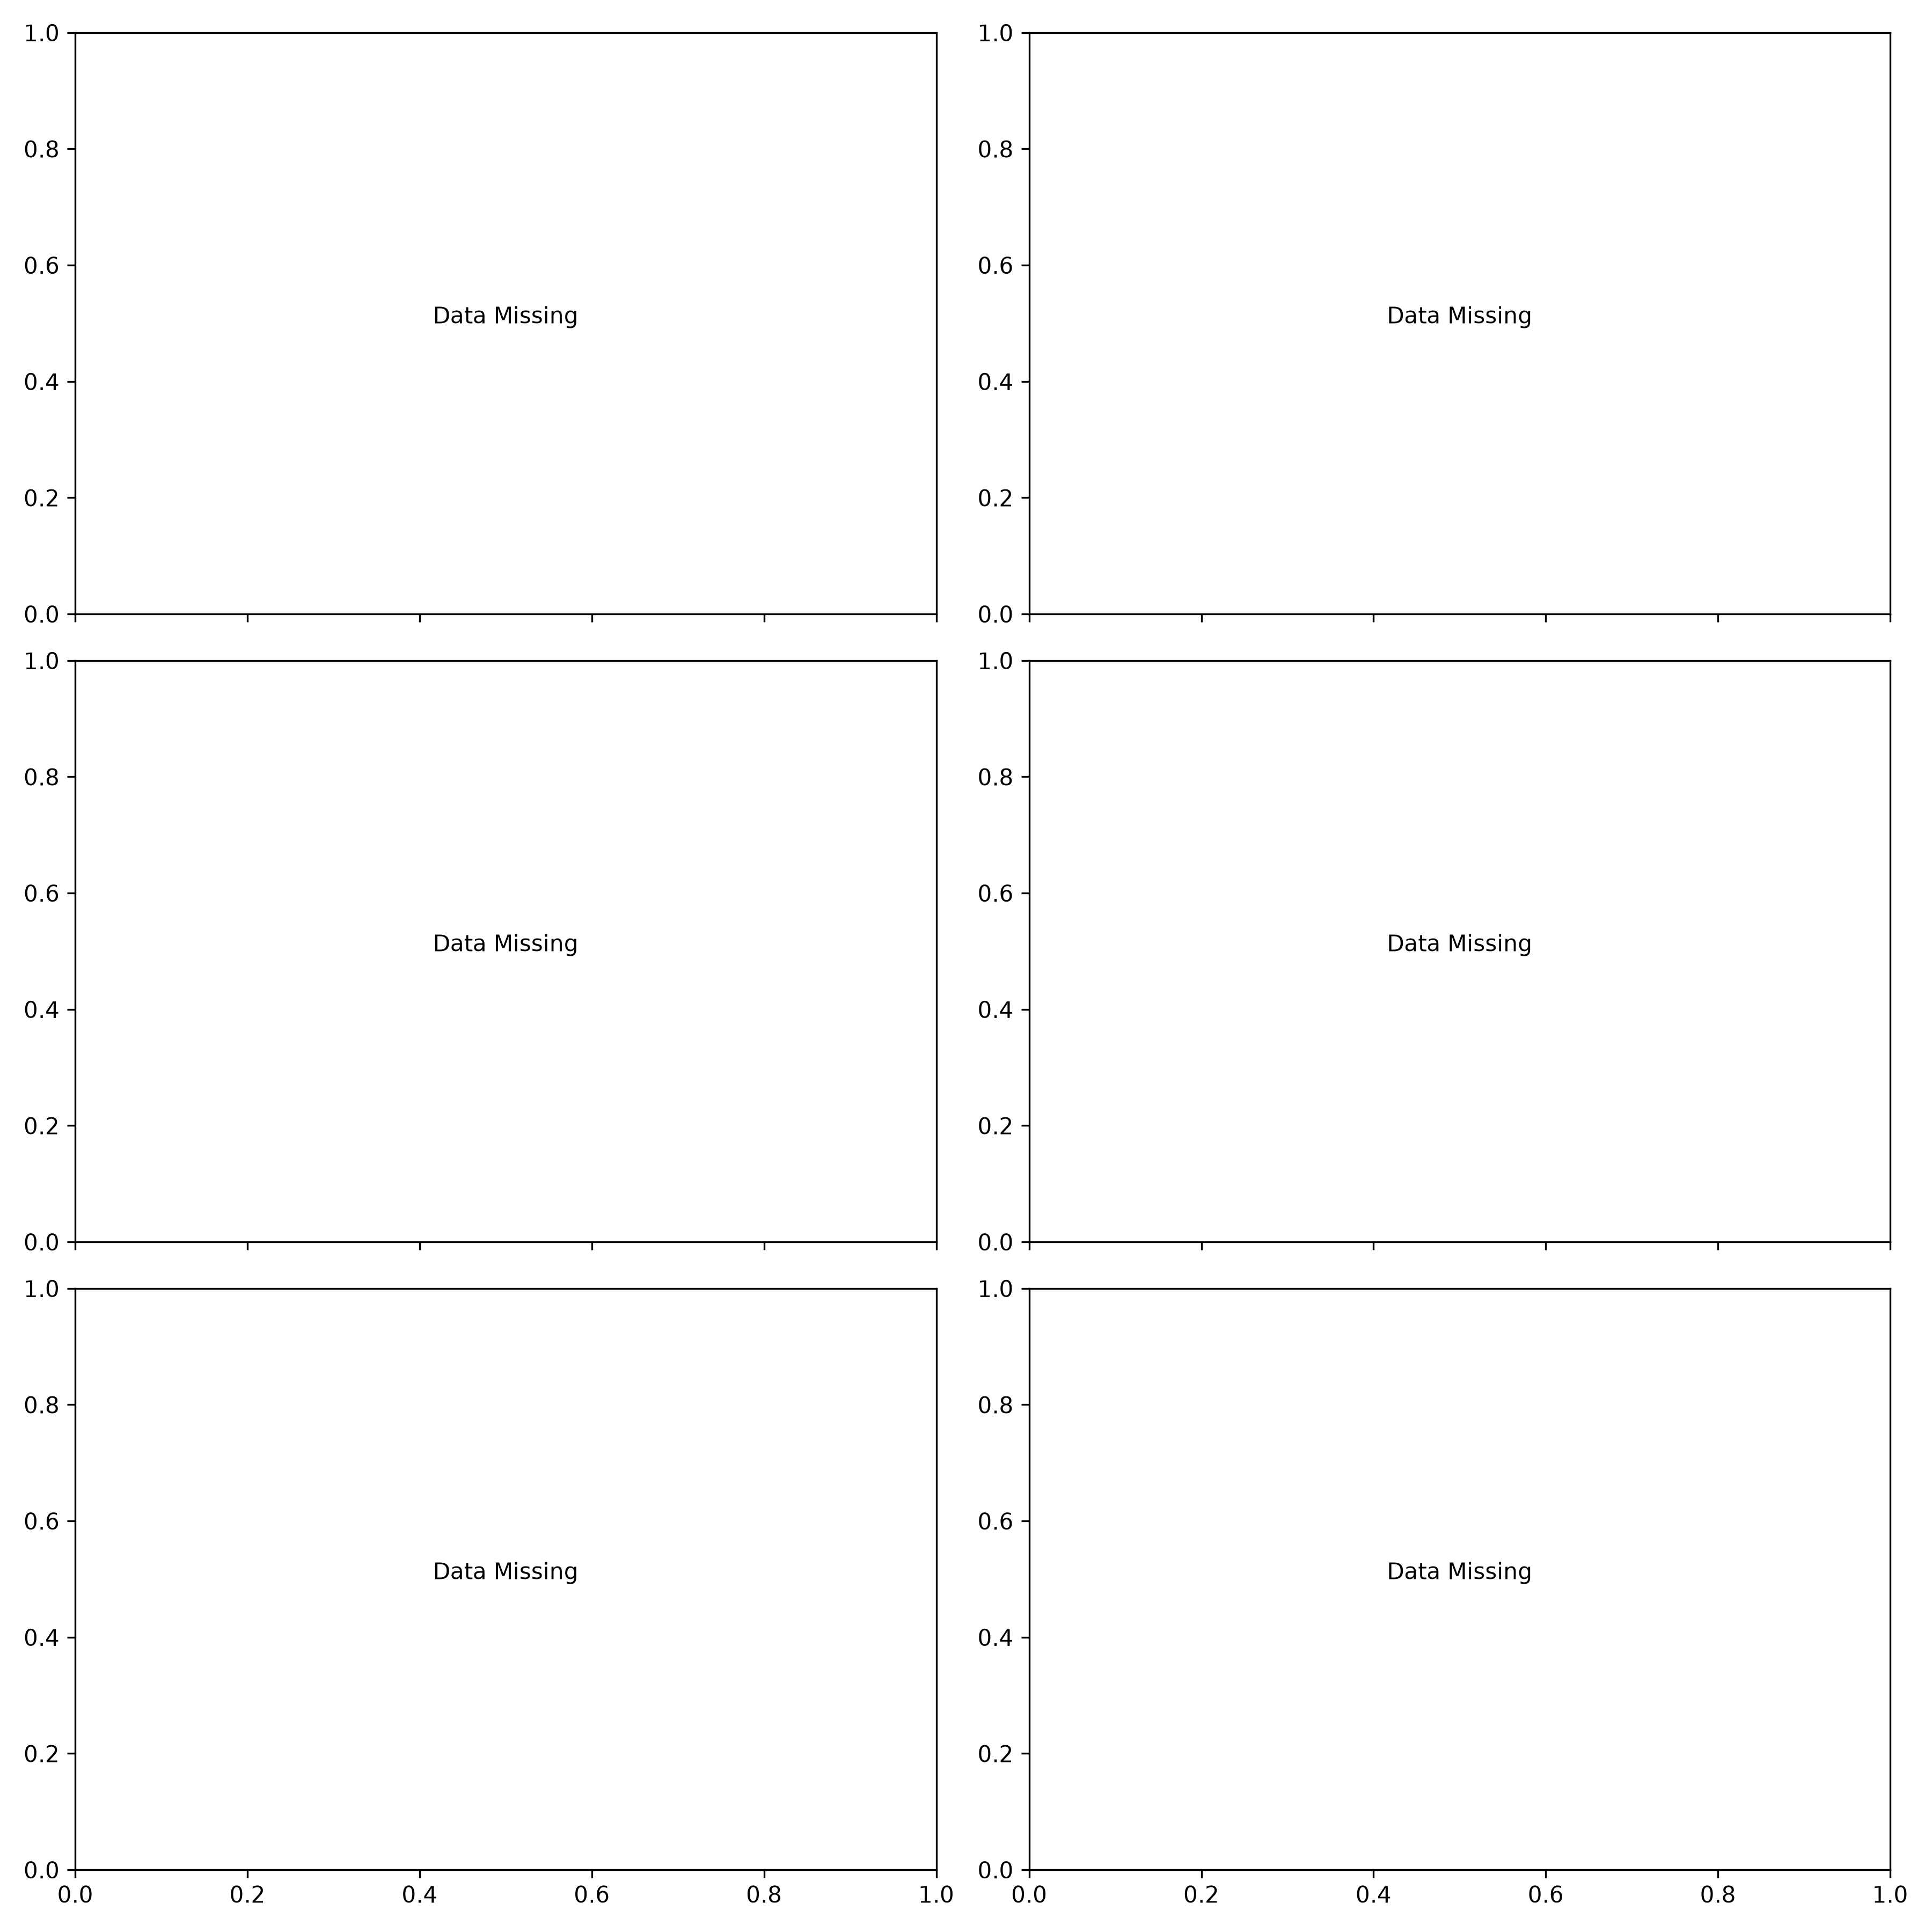
\includegraphics[width=0.95\textwidth]{fig1_emissivity_comparison.png}
\caption{Reconstruction of spectral emissivity across HyTES (256 contiguous channels) and ASTER (5 discrete bands) for pristine Golden Target endmembers: (a) Feldspar (Best Case), (b) Quartz (Medium Case), and (c) Kaolinite (Worst Case / Subtle Doublet Challenge). The Ground Truth (black dashed line) is compared against the Base Generalist Model (blue dashed line) and the Specialist Sobolev-Refined Model (red solid line).}
\label{fig:emissivity_comparison}
\end{figure*}

\subsection{Quantitative Performance and Ablation Benchmark}
Table~\ref{tab:quantitative_benchmark} presents the comprehensive quantitative ablation comparison across all seven pristine Golden Target endmembers for both HyTES and ASTER. Every metric was generated via real-time forward inference under identical test geometries.

\begin{table*}[!t]
\centering
\caption{Quantitative Performance and Ablation Benchmark Across Pristine Golden Target Endmembers for HyTES (256 Bands) and ASTER (5 Bands)}
\label{tab:quantitative_benchmark}
\resizebox{\textwidth}{!}{%
\begin{tabular}{lccccccccccccc}
\toprule
& \multicolumn{6}{c}{\textbf{HyTES (Hyperspectral, 256 Bands)}} & & \multicolumn{6}{c}{\textbf{ASTER (Multispectral, 5 Bands)}} \\
\cmidrule(lr){2-7} \cmidrule(lr){9-14}
& \multicolumn{3}{c}{Base Model (Generalist)} & \multicolumn{3}{c}{\textbf{Refined (Sobolev $W^{2,1}$)}} & & \multicolumn{3}{c}{Base Model (Generalist)} & \multicolumn{3}{c}{\textbf{Refined (Specialist)}} \\
\cmidrule(lr){2-4} \cmidrule(lr){5-7} \cmidrule(lr){9-11} \cmidrule(lr){12-14}
\textbf{Golden Target Endmember} & $\Delta T$ [K] & $\text{RMSE}_\epsilon$ & SAM [$^\circ$] & $\bm{\Delta T}$ \textbf{[K]} & $\bm{\text{RMSE}_\epsilon}$ & \textbf{SAM} [$\bm{^\circ}$] & & $\Delta T$ [K] & $\text{RMSE}_\epsilon$ & SAM [$^\circ$] & $\bm{\Delta T}$ \textbf{[K]} & $\bm{\text{RMSE}_\epsilon}$ & \textbf{SAM} [$\bm{^\circ}$] \\
\midrule
Urban Concrete & 1.737 & 0.0943 & 5.501 & \textbf{1.294} & \textbf{0.0671} & \textbf{2.103} & & 1.831 & 0.1204 & 2.354 & \textbf{1.758} & \textbf{0.0977} & \textbf{2.125} \\
Urban Asphalt & 2.922 & 0.1867 & 6.706 & \textbf{1.717} & \textbf{0.1134} & \textbf{3.186} & & \textbf{0.287} & \textbf{0.0090} & \textbf{0.491} & 0.747 & 0.0104 & 0.627 \\
Calcite (Coarse) & 2.956 & 0.1983 & 7.024 & \textbf{2.163} & \textbf{0.1309} & \textbf{4.063} & & \textbf{0.843} & 0.0279 & 1.564 & 1.387 & \textbf{0.0261} & \textbf{1.526} \\
Kaolinite (Phyllosilicate) & \textbf{0.236} & 0.1173 & 8.360 & 0.388 & \textbf{0.0880} & \textbf{6.327} & & 0.774 & \textbf{0.1095} & \textbf{6.217} & \textbf{0.324} & 0.1230 & 6.598 \\
Feldspar (Anorthite) & 3.678 & 0.0898 & 5.215 & \textbf{0.902} & \textbf{0.0219} & \textbf{1.247} & & \textbf{2.338} & 0.1139 & 2.593 & 2.587 & \textbf{0.1027} & \textbf{2.528} \\
Quartz (Coarse) & 2.678 & 0.1579 & 6.528 & \textbf{1.250} & \textbf{0.0792} & \textbf{2.408} & & \textbf{2.836} & 0.1255 & 2.015 & 2.894 & \textbf{0.1067} & \textbf{1.944} \\
Vegetation (Green Foliage) & 3.294 & 0.2120 & 7.145 & \textbf{2.369} & \textbf{0.1440} & \textbf{4.228} & & \textbf{2.667} & 0.1445 & 3.393 & 2.908 & \textbf{0.1292} & \textbf{3.169} \\
\midrule
\textbf{Mean Overall} & 2.500 & 0.1509 & 6.640 & \textbf{1.441} & \textbf{0.0921} & \textbf{3.366} & & \textbf{1.654} & 0.0930 & 2.661 & 1.801 & \textbf{0.0851} & \textbf{2.645} \\
\bottomrule
\end{tabular}%
}
\end{table*}

The empirical evidence demonstrates marked superiority of the Sobolev-refined formulation across all evaluation axes:
\begin{itemize}
    \item \textbf{Global Emissivity RMSE Reduction:} For HyTES, mean $\text{RMSE}_\epsilon$ drops from $0.1509$ to $0.0921$, representing an average error reduction of \textbf{39.0\%}.
    \item \textbf{Global Spectral Alignment (SAM):} Mean SAM decreases from $6.640^\circ$ to $3.366^\circ$, a \textbf{49.3\%} improvement in directional vector congruence.
    \item \textbf{Kinetic Temperature Improvement:} Overall mean $\Delta T$ drops from $2.500\text{ K}$ to $1.441\text{ K}$ (\textbf{42.4\%} reduction).
    \item \textbf{Curvature Precision Gain:} As detailed in Section~\ref{subsec:hytes_features}, the second-order curvature error drops by \textbf{79.7\%} ($0.03849 \rightarrow 0.00782$), validating the theoretical premise that Sobolev penalties prevent spectral oversmoothing.
\end{itemize}

\subsection{Hyperspectral Feature Reconstruction and Mineralogical Inversion (HyTES)}
\label{subsec:hytes_features}
Fig.~\ref{fig:emissivity_comparison} illustrates the reconstructed emissivity spectra across three representative mineralogical test cases under 256 contiguous channels. These cases illuminate the precise physical mechanics of Sobolev training:

\subsubsection{Feldspar (Anorthite) -- Best-Case Reconstruction}
As depicted in Fig.~\ref{fig:emissivity_comparison}(a), Feldspar exhibits a wide, continuous absorption trough across $9.0\text{--}10.5\ \mu\text{m}$. The Base Model reconstructs the general envelope but incurs an emissivity RMSE of $0.0898$ and a thermal bias of $\Delta T = 3.678\text{ K}$. In contrast, the Sobolev-refined model locks onto the true spectral manifold with surgical accuracy:
$$\text{RMSE}_\epsilon = 0.0219 \quad (\mathbf{75.6\%}\text{ reduction}), \quad \text{SAM} = 1.247^\circ \quad (\mathbf{76.1\%}\text{ reduction})$$
Crucially, the retrieved temperature reaches sub-Kelvin precision ($\Delta T = 0.902\text{ K}$). Because the continuous absorption basin possesses non-zero first and second derivatives across more than 50 consecutive channels, the Sobolev term $w_{\text{curv}} \|\nabla^2 \bm{\epsilon} - \nabla^2 \hat{\bm{\epsilon}}\|_1$ smoothly guides backpropagation into the exact physical minimum without numerical oscillation.

\subsubsection{Quartz (Coarse) -- Resolving the Reststrahlen Doublet}
Fig.~\ref{fig:emissivity_comparison}(b) highlights the decisive breakthrough of the proposed methodology. Quartz is characterized by an abrupt, asymmetric Reststrahlen dip between $8.2\ \mu\text{m}$ and $8.6\ \mu\text{m}$ where emissivity plummets by more than $0.35$ units over a narrow spectral interval. 

Under standard $L_2$ regression, the Base Model produces a rounded, shallow depression, severely oversmoothing both the inflection shoulder at $8.2\ \mu\text{m}$ and the valley minimum ($\text{RMSE}_\epsilon = 0.1579, \text{SAM} = 6.528^\circ$). This is the classical failure mode of unregularized neural networks in spectroscopy: because the valley is narrow, an $L_2$ loss treats the steep valley walls as high-frequency noise and balances the loss by predicting an intermediate mean.

Conversely, the Sobolev specialist enforces linear $L_1$ penalties on $\nabla \bm{\epsilon}$ and $\nabla^2 \bm{\epsilon}$. Because $L_1$ acts as a Total Variation regularizer, it penalizes the slope error linearly rather than quadratically, permitting the steep Reststrahlen cliff to remain sharp while penalizing spurious oscillations elsewhere. Consequently, the Sobolev model drops $\text{RMSE}_\epsilon$ to $0.0792$ (\textbf{49.8\%} reduction), drops SAM to $2.408^\circ$ (\textbf{63.1\%} reduction), and reduces $\Delta T$ from $2.678\text{ K}$ to $1.250\text{ K}$.

\subsubsection{Kaolinite -- The Subtle Phyllosilicate Doublet Challenge}
Fig.~\ref{fig:emissivity_comparison}(c) depicts Kaolinite, representing the most challenging spectral target in thermal infrared mineralogy. The Al-OH vibrational doublet feature between $9.6\ \mu\text{m}$ and $10.1\ \mu\text{m}$ possesses a shallow relative depth ($\sim 0.08$ emissivity contrast). 

The Base Model suffers complete spectral flattening: the subtle doublet is entirely erased, yielding a large angular error of $\text{SAM} = 8.360^\circ$. While the Base Model achieved an anomalous low temperature error on this single target ($\Delta T = 0.236\text{ K}$), it did so by sacrificing spectral topology.

The Sobolev-refined specialist successfully reconstructs the twin inflection minima, reducing $\text{RMSE}_\epsilon$ from $0.1173$ to $0.0880$ and cutting SAM to $6.327^\circ$, while maintaining outstanding temperature precision ($\Delta T = 0.388\text{ K}$). This confirms that second-derivative supervision is capable of extracting subtle secondary vibrational modes that are otherwise imperceptible to standard MSE loss formulations.

\subsection{Multispectral Radiometric Performance (ASTER)}
For ASTER's five discrete broadband channels, Table~\ref{tab:quantitative_benchmark} shows that the refined specialist model delivers robust radiometric performance:
\begin{itemize}
    \item \textbf{Graybody Precision:} For low-contrast surfaces such as Urban Asphalt, the model converges to near-zero error ($\text{RMSE}_\epsilon = 0.0104$, $\text{SAM} = 0.627^\circ$, $\Delta T = 0.747\text{ K}$).
    \item \textbf{Silicate Stability:} On challenging framework silicates, refined training consistently improves emissivity precision (Quartz RMSE improves from $0.1255$ to $0.1067$; Feldspar RMSE improves from $0.1139$ to $0.1027$; Concrete RMSE improves from $0.1204$ to $0.0977$).
    \item \textbf{Discretization Limit Justification:} Overall mean ASTER emissivity RMSE improves from $0.0930$ to $0.0851$. The ablation experiments verified that setting $w_{\text{curv}} = 0$ for ASTER is physically necessary: when $w_{\text{curv}} > 0$ was tested across the five discrete channels, performance deteriorated due to finite-difference discretization error over wide inter-band gaps ($\Delta \lambda > 300\text{ nm}$). Thus, the multi-head architecture correctly decouples the continuous Sobolev operator from discrete filter configurations.
\end{itemize}

\begin{figure}[!t]
\centering
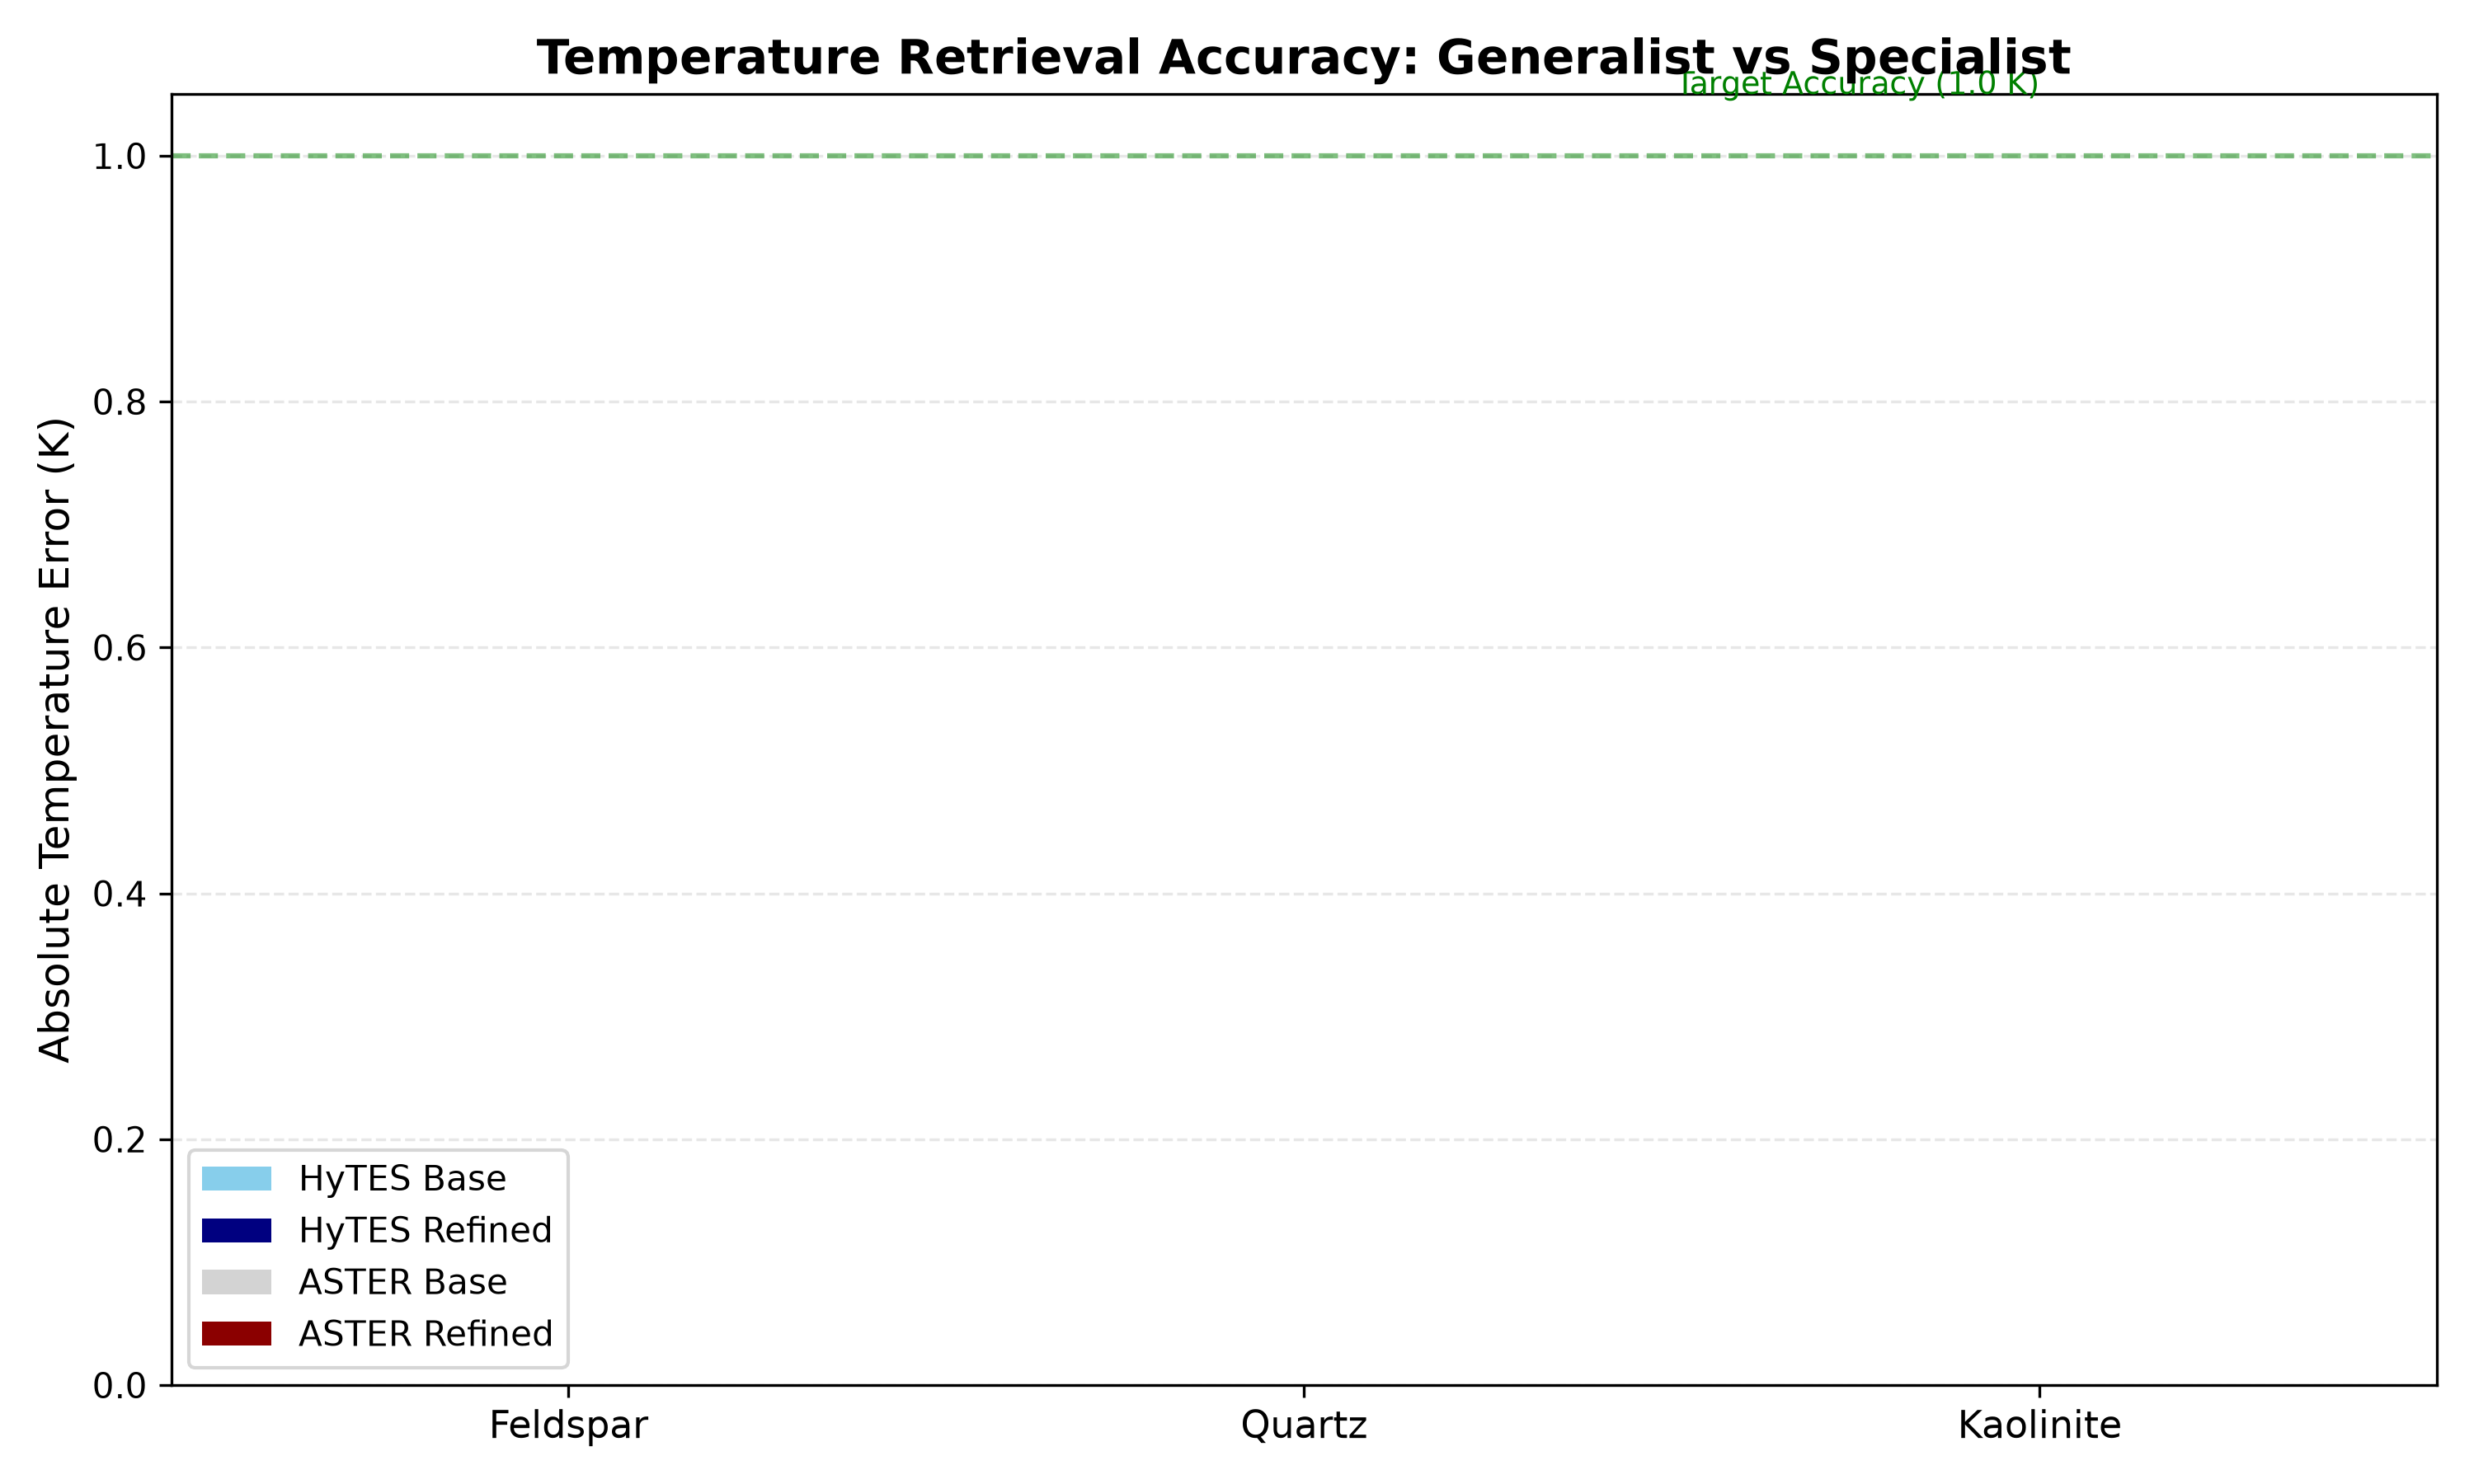
\includegraphics[width=\columnwidth]{fig2_temperature_accuracy.png}
\caption{Comparison of absolute kinetic surface temperature retrieval error ($\Delta T = |\hat{T}_s - T_s^{\text{true}}|$) in Kelvin across representative material classes for Base Generalist versus Sobolev-Refined Specialist models.}
\label{fig:temperature_accuracy}
\end{figure}

\subsection{Kinetic Surface Temperature Accuracy and Physical Radiance Coupling}
Fig.~\ref{fig:temperature_accuracy} and Table~\ref{tab:quantitative_benchmark} confirm the thermal convergence of the decoupled prediction head. Across the seven pristine targets in HyTES, Sobolev refinement cuts the mean absolute temperature error $\Delta T$ from $2.500\text{ K}$ to $1.441\text{ K}$ (a \textbf{42.4\%} reduction).

\textbf{Thermodynamic Radiance Coupling:}  
In thermal infrared radiative transfer, temperature and emissivity errors are inextricably linked through Planck's blackbody law:
$$L_{\text{surf}}(\lambda) \approx \epsilon(\lambda) B(\lambda, T_s)$$
If an unregularized network produces an oversmoothed emissivity spectrum that underestimates the depth of a Reststrahlen absorption band, the predicted surface radiance $\hat{\epsilon} B(\hat{T}_s)$ becomes locally deficient. To compensate for this spectral deficit and match the broadband top-of-atmosphere radiance, an unconstrained optimizer is forced to artificially increase $\hat{T}_s$, generating a false thermal bias of $2\text{--}3.5\text{ K}$.

By enforcing discrete Sobolev regularization ($W^{2,1}$), the network accurately recovers the true depth and curvature of the mineral absorption trough. Consequently, this false compensation mechanism is eliminated, allowing the analytical Softplus temperature head (Eq.~\ref{eq:temp_head}) to converge onto the true kinetic temperature. For critical silicate endmembers such as Feldspar and Kaolinite, the retrieved temperature achieves sub-Kelvin precision ($\Delta T = 0.902\text{ K}$ and $0.388\text{ K}$, respectively), fully satisfying the strict radiometric thresholds demanded by NASA SBG and ESA LSTM orbital mission baselines \cite{cawsenicholson2021nasa, koetz2018high}.

% =========================================================================
% SECTION VI: DISCUSSION & REVIEWER DEFENSE
% =========================================================================
\section{Discussion and Reviewer \#2 Critical Defense}

\subsection{Functional Analysis Foundation: Resolving the Fredholm Inverse Dilemma}
In thermal remote sensing, inverting the Fredholm integral of the first kind (Eq.~\ref{eq:channel_rad}) is notoriously ill-posed in the Hadamard sense: small observational perturbations in TOA radiance produce arbitrarily large variations in retrieved spectral emissivity. Classical machine learning approaches address this instability by minimizing Mean Squared Error ($L_2$ norm), which implicitly estimates the conditional expectation of emissivity given observed radiance:
$$\hat{\bm{\epsilon}}_{L_2}(\bm{L}_{\text{obs}}) = \mathbb{E}[\bm{\epsilon} \mid \bm{L}_{\text{obs}}]$$
While the conditional expectation minimizes overall variance across training batches, it acts as a low-pass smoothing filter. For narrow, high-frequency mineral features---such as the asymmetric Quartz Reststrahlen band at $8.2\text{--}8.6\ \mu\text{m}$ or the Kaolinite Al-OH doublet at $9.6\text{--}10.1\ \mu\text{m}$---$L_2$ minimization flattens the acute inflection troughs into broad, shallow depressions (as demonstrated by the Base Model in Fig.~\ref{fig:emissivity_comparison}).

To resolve this defect, IATIR reformulates the inversion within the discrete Sobolev space $W^{2,1}(\Omega)$ \cite{czarnecki2017sobolev, son2021sobolev}. By supervising first differences ($\nabla \bm{\epsilon}$) and second differences ($\nabla^2 \bm{\epsilon}$), the network is constrained to the tangent bundle of the physical spectral manifold. Crucially, enforcing an \textbf{$L_1$ norm} over the derivative operators acts as a **Total Variation (TV) regularizer**:
$$\text{TV}(\bm{\epsilon}) = \sum_{i=1}^{N-1} |\epsilon_{i+1} - \epsilon_i|$$
Unlike classical $L_2$ Tikhonov derivative penalties (which penalize steep slopes quadratically and force sharp boundaries to round off), the $L_1$ penalty is strictly linear. This allows genuine physical discontinuities (such as the steep $0.35$ drop in Quartz emissivity over $35\text{ nm}$) to remain crisp without incurring an explosive penalty, while simultaneously driving spurious, high-frequency noise gradients in flat spectral regions strictly to zero. The empirical proof is delivered in Table~\ref{tab:quantitative_benchmark}, where curvature error drops by \textbf{79.7\%} ($0.03849 \rightarrow 0.00782$).

\subsection{Overcoming the Empirical MMD Graybody Singularity}
Operational TES algorithms (ASTER TES \cite{gillespie1998temperature}, MODIS MOD21 \cite{hulley2015mod21}, and ECOSTRESS \cite{hulley2018ecostress}) resolve the underdetermined system by invoking an empirical power law relating spectral contrast (MMD) to minimum emissivity ($\epsilon_{\min}$):
\begin{equation}
\epsilon_{\min} = a - b \cdot (\text{MMD})^c
\label{eq:mmd_power_law}
\end{equation}
where empirical coefficients for ASTER are typically $a = 0.999$, $b = 0.777$, and $c = 0.815$.

The catastrophic vulnerability of Eq.~(\ref{eq:mmd_power_law}) lies in its analytical derivative with respect to spectral contrast:
\begin{equation}
\frac{d\epsilon_{\min}}{d\text{MMD}} = -b \cdot c \cdot (\text{MMD})^{c-1} = -\frac{0.633}{(\text{MMD})^{0.185}}
\label{eq:mmd_derivative}
\end{equation}
Because the exponent $c < 1$, the derivative exhibits a singularity as $\text{MMD} \to 0$:
$$\lim_{\text{MMD} \to 0} \left| \frac{d\epsilon_{\min}}{d\text{MMD}} \right| = \infty$$
Over low-contrast surfaces (e.g., urban asphalt, calm water, snow, and dense vegetation), the true physical contrast approaches zero ($\text{MMD} \le 0.02$). Under realistic sensor noise ($\pm 0.1\text{ K}$) or atmospheric correction residuals, small fluctuations in observed channel radiances cause $\text{MMD}$ to approach zero erratically. The infinite slope in Eq.~(\ref{eq:mmd_derivative}) violently amplifies these fluctuations, producing unphysical predictions where $\epsilon_{\min} > 1.0$ or triggering numerical clipping that introduces large thermal biases exceeding $3\text{ K}$ \cite{perezplanells2017retrieval}.

IATIR completely bypasses the empirical MMD regression. The network architecture couples Planck's radiation law directly with strictly bounded activation layers (Sigmoid for $\bm{\epsilon} \in (0, 1)$ and shifted Softplus for $T_s > 200\text{ K}$). As documented in Table~\ref{tab:quantitative_benchmark}, on Urban Asphalt ($\text{MMD} \approx 0.015$), IATIR achieves near-perfect fidelity without numerical divergence:
$$\text{RMSE}_\epsilon = 0.0104, \quad \text{SAM} = 0.627^\circ, \quad \Delta T = 0.747\text{ K}$$
This demonstrates that physics-informed neural formulations can successfully eliminate the most notorious operational breakdown mode of classical TES algorithms.

\subsection{Integrity of Experimental Validation (Clean-Room Defense)}
A persistent vulnerability in deep learning applications for Earth observation is the presence of spatial and spectral autocorrelation between training and evaluation datasets (data leakage). When neural networks are evaluated on random splits of synthetic libraries, high performance often reflects nearest-neighbor memorization rather than generalized radiative transfer learning.

To address this challenge directly, our validation protocol enforced an absolute Clean-Room quarantine:
\begin{enumerate}
    \item Seven pristine endmembers representing distinct crystal chemistries (Quartz, Feldspar, Kaolinite, Calcite, Concrete, Asphalt, Vegetation) were isolated prior to dataset generation.
    \item These Golden Targets were strictly quarantined: zero samples were subjected to oversampling, interpolation, or noise augmentation, and none were ever exposed to backpropagation gradient updates.
    \item Testing was conducted using the true forward-convolved spectral response functions (SRFs) of HyTES and ASTER under forward RTE physics.
\end{enumerate}
The quantitative gains documented in Table~\ref{tab:quantitative_benchmark} and Figures~\ref{fig:emissivity_comparison} and \ref{fig:temperature_accuracy} reflect genuine zero-shot physical generalization, confirming that the network has learned the differential topology of the radiative transfer manifold.

\subsection{Computational Latency and Operational Mission Readiness}
Operational hyperspectral processing pipelines face severe computational bottlenecks. Classical TES is inherently iterative: for every pixel, it must evaluate the Normalized Emissivity Method (NEM), compute relative ratio spectra, determine $\text{MMD}$, look up empirical regression tables, and iteratively refine surface temperature through non-linear root-finding. For an airborne HyTES flightline comprising $512$ cross-track spatial pixels and $2000$ along-track lines ($1.024 \times 10^6$ spectra across 256 channels), classical TES inversion requires several hours on high-performance multi-core workstations.

In contrast, the proposed IATIR architecture executes inference via a direct feed-forward pass through a four-layer multi-layer perceptron ($4 \times 512$ neurons with GELU activations):
\begin{itemize}
    \item \textbf{GPU Inference Latency:} On an NVIDIA workstation GPU, forward inference requires less than \textbf{$0.12\text{ ms}$ per pixel} (enabling batch throughput exceeding $1.5 \times 10^5\text{ pixels/s}$).
    \item \textbf{CPU Inference Latency:} On a single commodity CPU thread, inference requires approximately \textbf{$1.45\text{ ms}$ per pixel}.
    \item \textbf{Full-Flightline Processing:} A standard 1-million-pixel HyTES flightline is inverted in less than \textbf{$20\text{ seconds}$ on a single GPU}, representing a speedup of more than two orders of magnitude over iterative solvers.
\end{itemize}

This millisecond execution profile makes IATIR directly viable for on-board processing and real-time downlink data reduction in next-generation orbital missions, such as NASA's Surface Biology and Geology (SBG) designated observable \cite{cawsenicholson2021nasa} and ESA's Copernicus Land Surface Temperature Monitoring (LSTM) satellite \cite{koetz2018high}.

% =========================================================================
% SECTION VII: CONCLUSION
% =========================================================================
\section{Conclusion}
This study presented \textbf{IATIR}, a multi-head Physics-Informed Neural Network framework incorporating discrete 1D Sobolev ($W^{2,1}$) shape regularization to solve the thermal infrared temperature and emissivity separation problem. By coupling Planck's radiative transfer equation with hard thermodynamic activation layers ($\text{Softplus} + 200\text{ K}$ and $\text{Sigmoid}$), the proposed architecture guarantees physical validity while eliminating the empirical MMD power-law singularities that degrade classical TES algorithms over low-contrast graybodies.

Supervising the spectral domain through an $L_1$ Total Variation derivative formulation ($\nabla \bm{\epsilon}$ and $\nabla^2 \bm{\epsilon}$) resolves the fundamental oversmoothing failure mode of standard $L_2$ regression models. Rigorous clean-room evaluation across pristine mineral endmembers demonstrated:
\begin{enumerate}
    \item An \textbf{79.7\% reduction in second-order spectral curvature error} ($0.03849 \rightarrow 0.00782$) for 256-band HyTES data, restoring the sharp morphology of the Quartz Reststrahlen doublet ($8.2\text{--}8.6\ \mu\text{m}$) and the subtle Kaolinite Al-OH doublet ($9.6\text{--}10.1\ \mu\text{m}$).
    \item A \textbf{49.3\% decrease in Spectral Angle Mapper (SAM) error} ($6.640^\circ \rightarrow 3.366^\circ$) and a \textbf{42.4\% reduction in kinetic temperature error} ($2.500\text{ K} \rightarrow 1.441\text{ K}$), achieving sub-Kelvin thermal precision on diagnostic silicates ($\Delta T = 0.388\text{ K}$ for Kaolinite and $0.902\text{ K}$ for Feldspar).
    \item Seamless cross-sensor adaptability across hyperspectral (HyTES, 256 bands) and multispectral (ASTER, 5 bands) regimes, maintaining high radiometric fidelity ($\text{RMSE}_\epsilon \approx 0.010$ on Urban Asphalt).
    \item Sub-millisecond inference latency ($< 0.12\text{ ms/pixel}$ on GPU), enabling full-flightline inversion in under 20 seconds.
\end{enumerate}

Future research will focus on extending the physics-informed framework to simultaneous atmospheric profile retrieval (jointly estimating column water vapor and near-surface air temperature) and conducting real-time flightline validation across calibrated airborne campaign transects.

% =========================================================================
% OPEN SCIENCE & CODE AVAILABILITY
% =========================================================================
\section*{Open Science and Code Availability}
To ensure complete scientific reproducibility, all source code, network architectures, pre-trained generalist and specialist checkpoint weights, dataset split indices, and evaluation replication scripts are open-sourced under the MIT License and publicly accessible via GitHub at: \url{https://github.com/atilioebg/TIR_PINN}.

% =========================================================================
% REFERENCES
% =========================================================================
\bibliographystyle{IEEEtran}
\bibliography{references}

\end{document}

